%%% Template originaly created by Karol Kozioł (mail@karol-koziol.net) and
%%% modified for ShareLaTeX use

\documentclass[a4paper,12pt]{article}

\usepackage[
  backend=biber,
  style=authoryear-ibid, % Motsvarar agsm.
  uniquename=init,
  giveninits,  % Ersätt hela förnamn med bara initialerna.
  maxnames=2,  % Ersätt med et al./m.fl. om det är fler än två förf.
  natbib=true,
  hyperref=true,
  % backref=true,
  doi=false,
  isbn=false,
  url=false
]{biblatex}
\addbibresource{report.bib}
% Lite kortare referenslista utan URL:er och DOI:er.

\usepackage[utf8]{inputenc}
\usepackage{csquotes} % Must be before babel.
\usepackage[english]{babel}
\usepackage[T1]{fontenc}
\usepackage{pdfsync}
\synctex=1
\usepackage{parskip} % Package to tweak paragraph skipping.
\usepackage{hyperref}
\usepackage{xcolor}

\usepackage{fancyhdr}

\renewcommand\familydefault{\sfdefault}
\usepackage{tgheros}
\usepackage[framed,numbered]{matlab-prettifier}
\makeatletter
\newcommand\BeraMonottfamily{%
  \def\fvm@Scale{0.6}% scales the font down
  \fontfamily{fvm}\selectfont% selects the Bera Mono font
}
\makeatother

\usepackage{amsmath,amssymb,amsthm,textcomp}
\usepackage{enumerate}
\usepackage{multicol}
\usepackage{tikz}
\usepackage{caption,subcaption}
\captionsetup[figure]{labelfont=bf,textfont=it}

\usepackage{calc}
\newenvironment{altDescription}[1][\quad]
  {\begin{list}{}{
   \renewcommand\makelabel[1]{\hfil\textsf{##1}}
   \settowidth\labelwidth{\makelabel{#1}}
   \setlength\leftmargin{\labelwidth+\labelsep}}}
  {\end{list}}
\usepackage{titling}

\title{AI for Game Programming 2: Maze Generation (A3.6)}
\author{Jonas Nockert}
% \renewcommand{\maketitlehookb}{\centering Description}
\date{\small January 8, 2020}

\begin{document}

\maketitle

\section*{Basic steps: Maze generation on a Voronoi diagram}
See figures \ref{fig:dots}, \ref{fig:delaunay}, \ref{fig:circumcenters},
\ref{fig:voronoi}, \ref{fig:maze} and \ref{fig:maze-connections}.

\section*{Growing Tree using the gamma distribution for branching}
The Recursive Backtracker algorithm consists of the following steps

\begin{enumerate}
  \item Add a starting cell to an empty stack, marking the cell as visited,
  \item pop a cell of the top of the stack,
  \item find a non-visited neighbor to that cell (or step 7 in case none exists,)
  \item remove the edge between this neighbor and cell,
  \item re-add the cell to the top of the stack in case there are more neighbors,
  \item add the neighbor to the top of the stack, marking it as visited,
  \item return to step 2 until the queue is empty.
\end{enumerate}

The growing tree algorithm is a variation of the above regarding how the
next cell is picked in step 2. If the growing tree algorithm is
set to always choose the most recently added cell, it becomes equivalent to
Recursive Backtracking or depth-first search (see
figure~\ref{fig:maze-dfs}). If cells are chosen at random,
it becomes equivalent to Prim's algorithm (a minimum spanning tree of a graph can
be viewed as a maze). Another option is to pick the oldest cells in the queue,
essentially breadth-first search, which tends to create long straight corridors
and not good mazes (see figure~\ref{fig:maze-bfs}).

It seems that often a ratio is picked between two or more of the above cases,
e.g. randomly picking most recent or by random in a 50/50 split.

Here, for variation, choices are sampled according to the gamma distribution
which can be seen as the picks are done with some regularity in terms
of rate of occurence. I've chosen to pick the oldest cells with a mean
of every sixth time with most recent cells picked in between.

The idea (hope) is that this will lead to longer winding dead-end branches
off the "main" path but with a guarantee that there's always some winding
segments between branches as the gamma distribution is positive valued.
The branches should not be allowed to compete too much for space in order
for both branches and main path to achieve a degree of windingness.

The benefit is longer dead-end corridors but the downside is that the
longest path generated is shorter than what Recursive Backtracker algorithm
would produce. This is inherent in the trade-off between DFS and BFS.

Examples of mazes generated by this algorithm is shown in
figures~\ref{fig:maze-gamma-mix}~and~\ref{fig:maze-uniform}.


\begin{figure}[ht]
  \centering
  \includegraphics[width=\linewidth]{images/dots.png}
  \caption{From a number of points arranged (semi-randomly) on a grid…
  \label{fig:dots}}
\end{figure}

\begin{figure}[ht]
  \centering
  \includegraphics[width=\linewidth]{images/delaunay.png}
  \caption{…a Delaunay triangulation is created using the procedure
    described in \citep{Yonghe:2013}. Turns out that simple is relative.
    In order to become Delaunay, the triangulation needs to be Lawson
    legalized, which I struggled with for a long time.
  \label{fig:delaunay}}
\end{figure}

\begin{figure}[ht]
  \centering
  \includegraphics[width=\linewidth]{images/circumcenters.png}
  \caption{The Delaunay triangulation is dual with its Voronoi diagram so
    the latter can be created from the former. Each triangle has a circumcenter (pink).
  \label{fig:circumcenters}}
\end{figure}

\begin{figure}[ht]
  \centering
  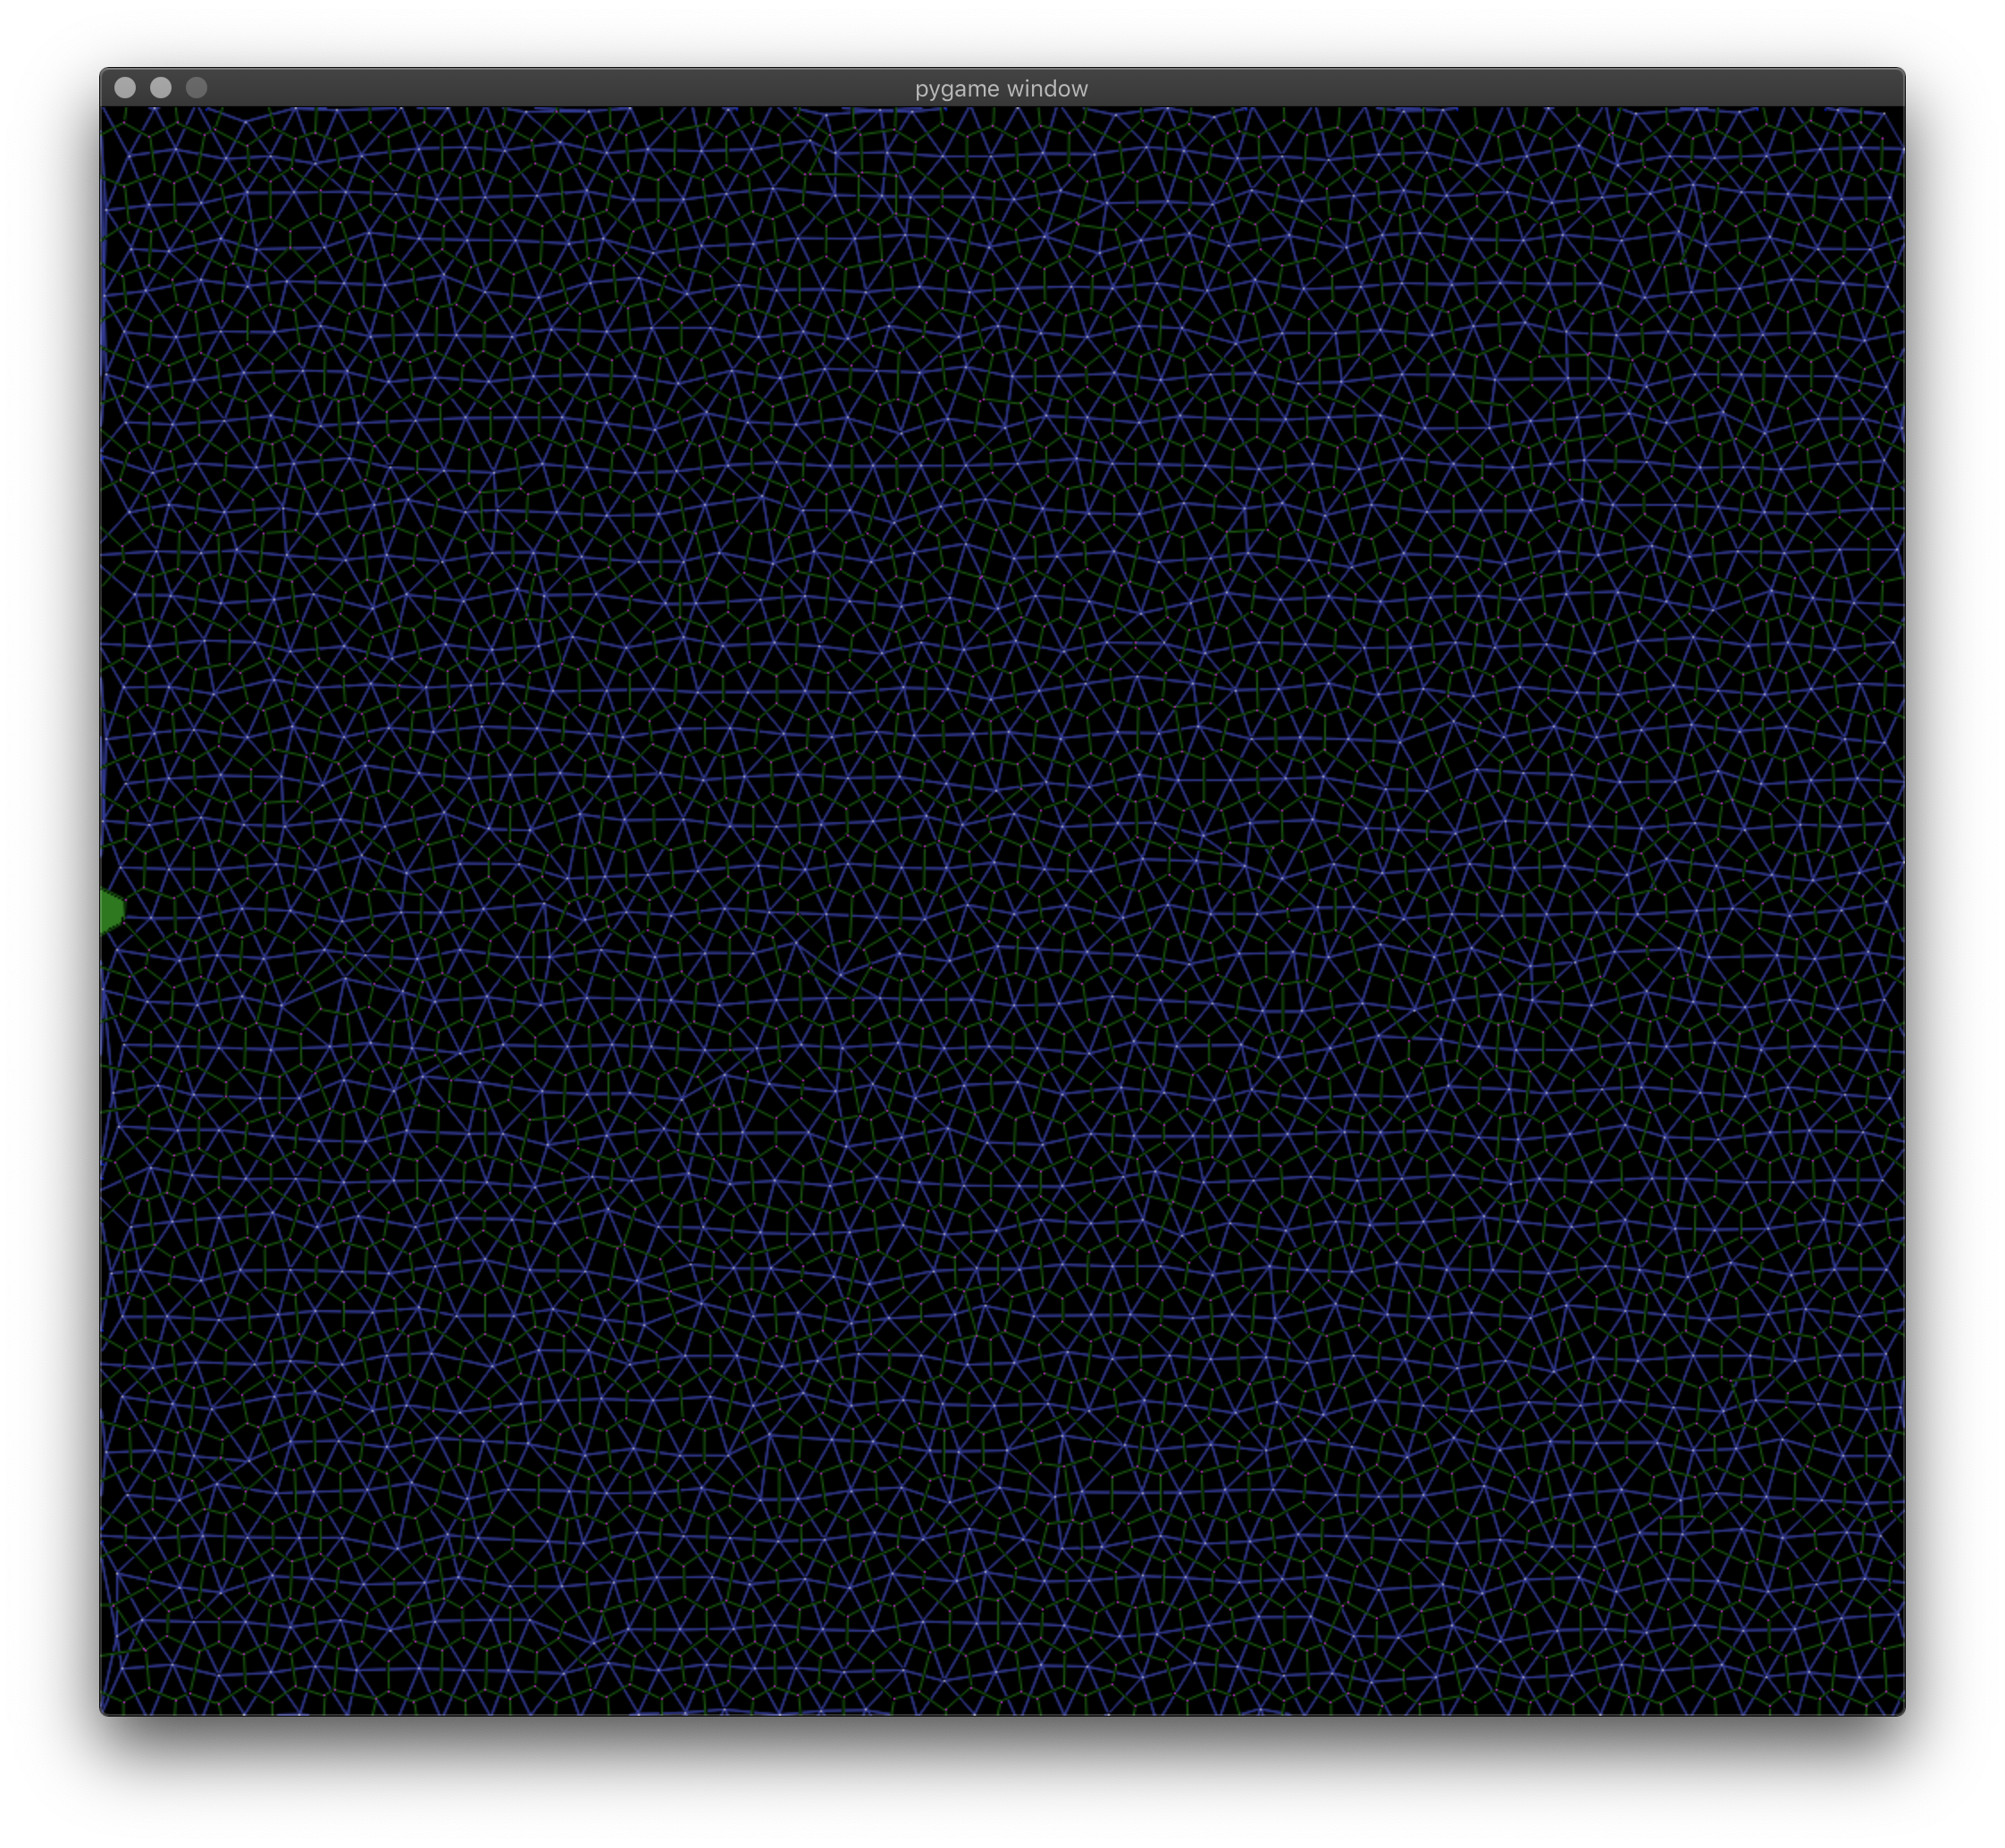
\includegraphics[width=\linewidth]{images/voronoi.png}
  \caption{Edges between the circumcenters of adjacent triangles can be
    connected into cells. Starting with an edge and following edges
    counterclockwise until the edge one started with is reached
    again we have acquired the polygon of a single cell. Each
    cell can have up to six neighbor cells.
  \label{fig:voronoi}}
\end{figure}

\begin{figure}[ht]
  \centering
  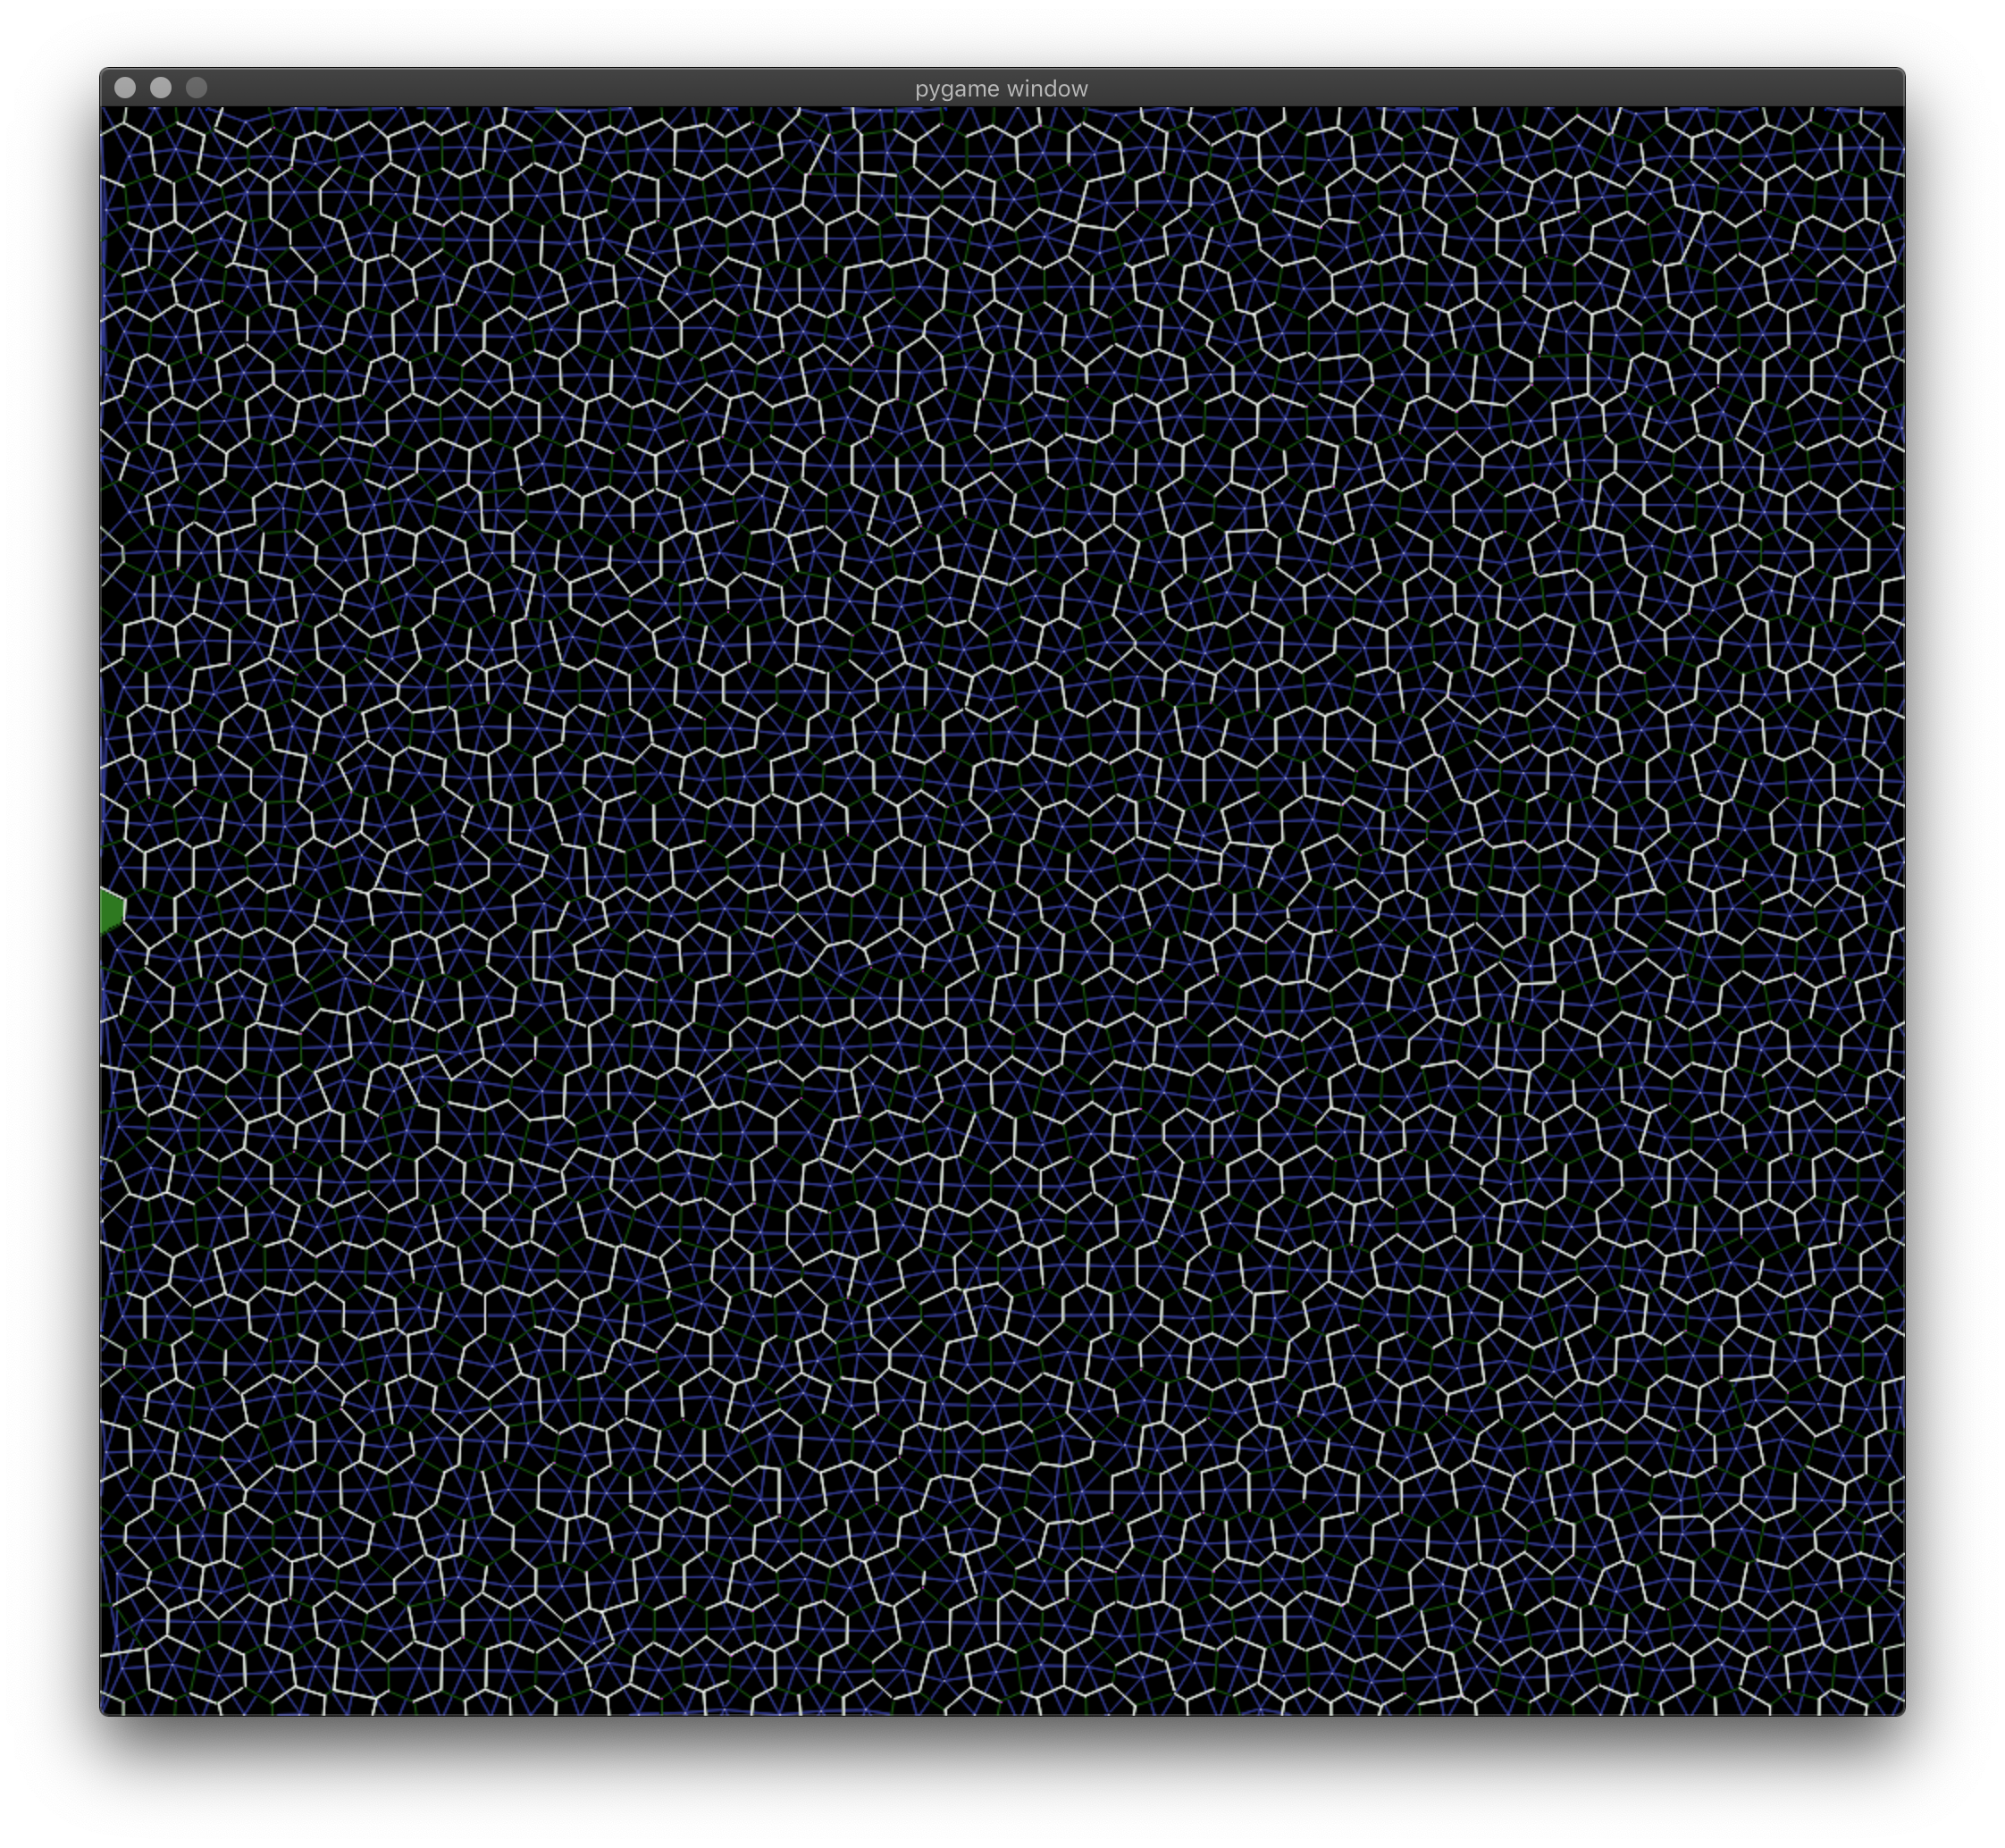
\includegraphics[width=\linewidth]{images/voronoi-maze.png}
  \caption{Although the Recursive Backtracker and Growing Tree algorithms are
    typically shown with square grids, they work on >4-sided polygons as well.
    Here we see the resulting maze after cell edges has been removed using a
    variation of the Growing Tree algorithm.
  \label{fig:maze}}
\end{figure}

\begin{figure}[ht]
  \centering
  \includegraphics[width=\linewidth]{images/voronoi-maze-connections.png}
  \caption{Since openings between cells can be narrow due to randomness in
    initial point placement, it can be difficult to see how they are connected.
    Here the maze paths are shown in cyan.
  \label{fig:maze-connections}}
\end{figure}

\begin{figure}[ht]
  \centering
  \includegraphics[width=0.7\linewidth]{images/maze-dfs.png}
  \includegraphics[width=0.7\linewidth]{images/maze-dfs-connections.png}
  \caption{Using the Recursive Backtracker algorithm (essentially depth-first
    search) to generate mazes tends to lead to one long, winding corridor with
    short dead end corridors branching off. This is equivalent to using the
    Growing Tree algorithm while always picking the cell on top of the stack
    (i.e. most recently added cells).
  \label{fig:maze-dfs}}
\end{figure}

\begin{figure}[ht]
  \centering
  \includegraphics[width=0.7\linewidth]{images/maze-bfs.png}
  \includegraphics[width=0.7\linewidth]{images/maze-bfs-connections.png}
  \caption{Using breadth-first search to generate mazes, not surprisingly, tends to
    lead to the opposite. Here we get many, mostly straight, corridors competing
    for the space.
  \label{fig:maze-bfs}}
\end{figure}

\begin{figure}[ht]
  \centering
  \includegraphics[width=0.7\linewidth]{images/maze-gamma.png}
  \includegraphics[width=0.7\linewidth]{images/maze-gamma-connections.png}
  \caption{Combining DFS and BFS seems to be a good idea. However, instead of just
    mixing the two randomly, I wanted to do it with some regularity. My idea
    was to use the gamma distribution to model the rate of branching, which
    guarantees spacing in between branches and should allow for winding and length
    in both main path as well as branches. The gamma distribution also means
    branches will occur regularly (but not too regularly).
  \label{fig:maze-gamma-mix}}
\end{figure}

\begin{figure}[ht]
  \centering
  \includegraphics[width=0.7\linewidth]{images/maze-uniform.png}
  \includegraphics[width=0.7\linewidth]{images/maze-uniform-connections.png}
  \caption{An example of a maze generated by the algorithm with initial points placed
    by sampling coordinates uniformly at random rather than on a semi-regular grid.
  \label{fig:maze-uniform}}
\end{figure}

\printbibliography{}
\end{document}
